\chapter{Spezifikation}

\section{Resourcen}
\label{sec:specification-resources}

Als Thema der API haben wir uns für einen einfachen Internet-Blog entschieden.
In diesem Blog sollen Benutzer (\texttt{User}) Blog-Artikel (\texttt{Posts}) schreiben können und unter Artikeln Kommentare (\texttt{Comments}) verfassen können. 

Daraus bilden wir ein Datenbank \ac{ER}-Diagram (siehe \ref{fig:blog-er-diagram})

\begin{figure}[hbp]
\centering
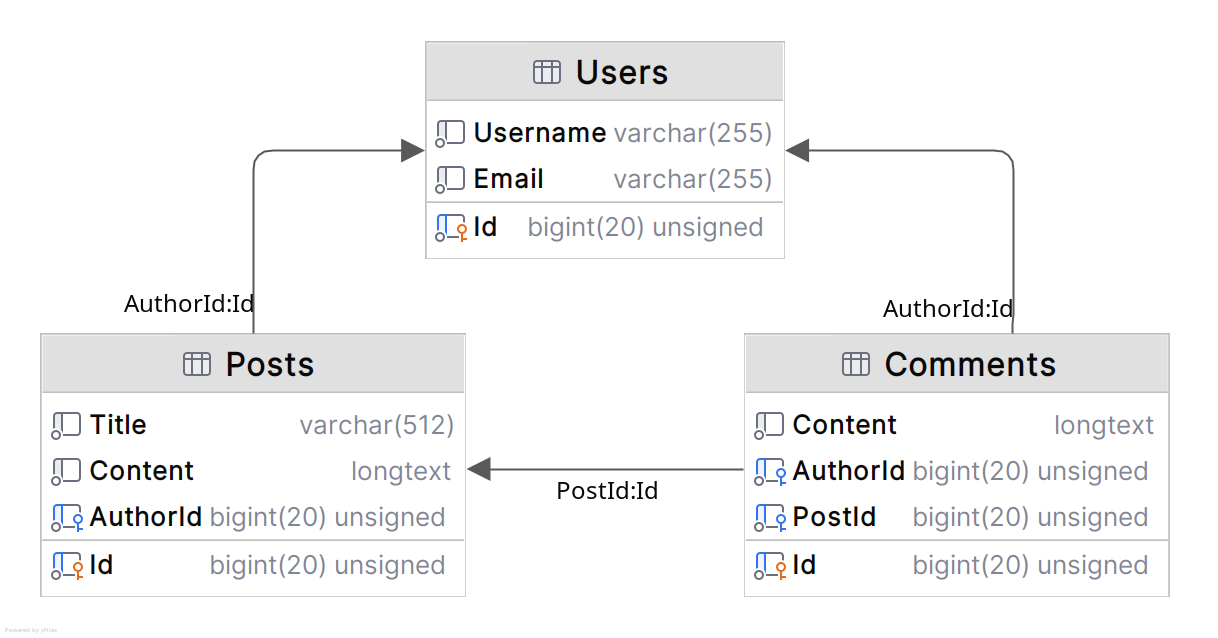
\includegraphics[width=0.8\linewidth]{Graphics/Database_ER.png}
\caption{ER-Diagram}
\label{fig:blog-er-diagram}
\end{figure}

Die einzelnen Entities verwenden wir um daraus Resourcen der REST-API (und damit die Models und \ac{DTO}) zu bauen.

\subsection{Modelle}
\label{subsec:specification-resources-models}

Die Modelle sind vollständig ersichtlich aus dem \ac{ER}-Diagramm (siehe \ref{fig:blog-er-diagram}). Hier werden nur zusätzlich Einschränkungen zu den Eigenschaften der Modelle festgelegt. Beispielsweise muss die E-Mail eines Nutzers dem E-Mail-Format entsprechen. Daraus ergibt sich für jede Entity ein validierbares Schema, welches in der API verwendet werden kann.

\section{OpenAPI}

\textit{Die OpenAPI-Spezifikation ist unter dem Pfad} \textbf{docs/specification.yaml} \textit{zu finden.}\\

Zur Spezifikation unserer REST-API benutzen wir die \textbf{OpenAPI}\footnote{\url{https://www.openapis.org}} Spezifikation.
Mit diesem Standard ist es möglich die Struktur (Endpunkte) und das Verhalten (Antwortmöglichkeiten- und Formate, Authentifizierung, etc) zu spezifizieren.
Dies geschieht wahlweise im Format \texttt{JSON} oder \texttt{YAML}, damit ist es maschinell lesbar.

\subsection{Vorgehen}

Da die Resourcen feststehen (siehe \ref{sec:specification-resources}) sind die Endpunkte der REST-API entsprechend einfach zu spezifizieren. 

Pro Resource (beispielsweise unter \texttt{/resource}) gibt es 5 Endpunkte:
\begin{itemize}
    \item \textbf{GET} \texttt{/resource}: Rufe alle Elemente dieser Resource ab.
    \item \textbf{POST} \texttt{/resource}: Erstelle ein neues Element dieser Resource.
    \item \textbf{GET} \texttt{/resource/\{id\}}: Rufe das Element mit der ID \texttt{\{id\}} ab.
    \item \textbf{PUT} \texttt{/resource/\{id\}}: Aktualisiere das Element mit der ID \texttt{\{id\}}.
    \item \textbf{DELETE} \texttt{/resource/\{id\}}: Lösche das Element mit der ID \texttt{\{id\}}.
\end{itemize}

Zu jedem dieser Endpunkte spezifizieren wir das Anfrageschema und die möglichen Antwortschemata. Hier sind dies beispielsweise folgende mögliche Antworten:

\begin{itemize}
    \item \textbf{200} \texttt{OK}: Anfrage ist erfolgreich verarbeitet.
    \item \textbf{400} \texttt{Bad Request}: Anfrage ist fehlerhaft.
    \item \textbf{403} \texttt{Unauthorized}: Anfrage ist nicht authentifiziert.
\end{itemize}

Wir können weitere Meta-Daten zu diesen Endpunkten angeben, wie zum Beispiel eine kurze Zusammenfassung, die Authentifizierungsanforderungen oder Gruppierungen.

\subsection{Möglichkeiten der OpenAPI-Spezifikation}
Eine vollständige OpenAPI-Spezifikation kann in meheren Bereichen eingesetzt werden. 
Im folgenden eine kurze, unvollständige Auflistung der Möglichkeiten.

Für eine größere Liste an Möglichkeiten, siehe \url{https://openapi.tools/}

\subsubsection*{Code-Generation}

Mit OpenAPI-Generators\footnote{\url{https://github.com/OpenAPITools/openapi-generator}} kann man sich Clients, Server Stubs, Tests oder Dokumentation generieren lassen.

Beispiele für generierte Ausgaben der OpenAPI-Generators für dieses Projekt sind zu finden unter:
\begin{itemize}
    \item \texttt{docs/openapi-generated-html1}: HTML-Dokumentation 1
    \item \texttt{docs/openapi-generated-html2}: HTML-Dokumentation 2
    \item \texttt{docs/openapi-generated-markdown}: Markdown-Dokumentation
    \item \texttt{openapi-generated-jaxrs-jersey}: Jersey Server Stubs
    \item \texttt{openapi-generated-java-client}: Java API Client
    \item \texttt{openapi-generated-aspnetcore}: ASP.NET Core Server Stubs
\end{itemize}

\subsubsection*{Mock-Server}

Es gibt verschiedene Services, welche eine Spezifikation dazu verwenden Standardantworten zurückzusenden. Dies funktioniert auch ohne Serverimplementation.
